\documentclass[12pt]{article}

% Pretty much all of the ams maths packages
\usepackage{amsmath,amsthm,amssymb,amsfonts}

% Allows you to manipulate the page a bit
\usepackage[a4paper]{geometry}

% Pulls the page out a bit - makes it look better (in my opinion)
\usepackage{a4wide}

% Removes paragraph indentation (not needed most of the time now)
\usepackage{parskip}

% Allows inclusion of graphics easily and configurably
\usepackage{graphicx}

% Provides ways to make nice looking tables
\usepackage{booktabs}

% Allows you to rotate tables and figures
\usepackage{rotating}

% Allows shading of table cells
\usepackage{colortbl}
% Define a simple command to use at the start of a table row to make it have a shaded background
\newcommand{\gray}{\rowcolor[gray]{.9}}

\usepackage{textcomp}

% Provides commands to make subfigures (figures with (a), (b) and (c))
\usepackage{subfigure}

% Typesets URLs sensibly - with tt font, clickable in PDFs, and not breaking across lines
\usepackage{url}

% Makes references hyperlinks in PDF output
\usepackage{hyperref}

% Provides ways to include syntax-highlighted source code
\usepackage{listings}
\lstset{frame=single, basicstyle=\ttfamily}

% Provides Harvard-style referencing
\usepackage{natbib}
\bibpunct{(}{)}{;}{a}{,}{,}

% Provides good access to colours
\usepackage{color}
\usepackage{xcolor}

\usepackage{tikz}

% Simple command I defined to allow me to mark TODO items in red
\newcommand{\todo}[1] {\textbf{\textcolor{red}{#1}}}

% Allows fancy stuff in the page header
\usepackage{fancyhdr}
\pagestyle{fancy}

% Vastly improves the standard formatting of captions
\usepackage[margin=10pt,font=small,labelfont=bf, labelsep=endash]{caption}

% Standard title, author etc.
\title{Report: Spanning USA}
\author{by	Mikkel Bernt Buchvardt and Theodor Lars Nyholm Ommen}
\date{}
% Put text on the left-hand and right-hand side of the header
\fancyhead{}
\lhead{Spanning USA}
\rhead{Buchvardt - Ommen}
\chead{}

\usepackage{titletoc}

\renewcommand{\thepart}{\Alph{part}}

\renewcommand{\thesection}{\arabic{section}}
\renewcommand{\thesubsection}{\alph{subsection})}
\renewcommand{\thesubsubsection}{\alph{subsection}\alph{subsubsection})}

\titlecontents{chapter}
[2.65em]
{\addvspace{10pt}\bfseries}
{\contentslabel{2.3em}}
{\hspace*{-2.3em}}
{\space.\hfill\contentspage}


\definecolor{dkgreen}{rgb}{0,0.6,0}
\definecolor{gray}{rgb}{0.5,0.5,0.5}
\definecolor{mauve}{rgb}{0.58,0,0.82}

\lstset{frame=tb,
	language=Java,
	aboveskip=3mm,
	belowskip=3mm,
	showstringspaces=false,
	columns=flexible,
	basicstyle={\small\ttfamily},
	numbers=left,
	numberstyle=\tiny\color{gray},
	keywordstyle=\color{blue},
	commentstyle=\color{dkgreen},
	stringstyle=\color{mauve},
	breaklines=true,
	breakatwhitespace=true,
	tabsize=3
}






\begin{document}
  \maketitle

%
\includegraphics[scale=0.55]{frontpage}

  \section{Results}

  The following table summarizes our result:
  
    \bigskip\noindent
  \begin{tabular}{lr}
  	\toprule
  	Input file & MST total weight \\ \midrule
  	USA-highway-miles.txt	 & 16598.0 \\
  	tinyEWG-alpha.txt & 181 \\ \bottomrule
  \end{tabular}
  
    \bigskip
  
     The MST we found in tinyEWG-alpha.txt can be drawn like this:
     
     
     
     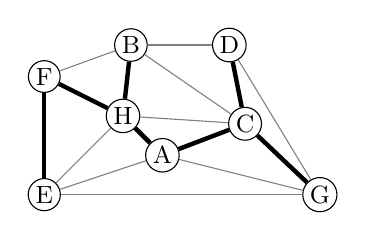
\begin{tikzpicture}[
     scale = .5,
     every node/.style = {
     	circle, draw, black, inner sep = 1pt, font = \small},
     every path/.style = {gray}
     ]
     
       \node (A) at (3,1) {A}; % 0
       \node (B) at (2.2,3.8) {B}; % 1
       \node (C) at (5.1,1.8) {C}; % 2
       \node (D) at (4.7,3.8) {D}; % 3
       \node (E) at (0,0) {E}; % 4
       \node (F) at (0,3) {F}; % 5
       \node (G) at (7,0) {G}; % 6
       \node (H) at (2,2) {H}; % 7
       \draw (E)--(F);
       \draw (E)--(H);
       \draw (F)--(H);
       \draw (A)--(H);
       \draw (B)--(F);
       \draw (A)--(E);
       \draw (C)--(D);
       \draw (B)--(H);
       \draw (A)--(C);
       \draw (B)--(C);
       \draw (B)--(D);
       \draw (C)--(H);
       \draw (G)--(C);
       \draw (D)--(G);
       \draw (G)--(A);
       \draw (G)--(E);
       \begin{scope}[every path/.style={ultra thick}]
       \draw(A)--(H);
       \draw(B)--(H);
       \draw(A)--(C);
       \draw(C)--(D);
       \draw(F)--(H);
       \draw(E)--(F);
       \draw(G)--(C);
       \end{scope}
     
     
     
     
      \end{tikzpicture}
      
  
  
  The MST has the following edges (lenghts in drawing are not correct):
  
  A - H weight: 16.0
  
  B - H weight: 19.0
  
  A - C weight: 26.0
  
  C - D weight: 17.0
  
  F - H weight: 28.0
  
  E - F weight: 35.0
  
  G - C weight: 40.0
  
  Total lenght of MST: 181.0 
  
  \section{Implementation details}

  We implemented the algorithms from the book page: 
  
  LazyPrimMST.java using MinPQ.java. The total running time is E*log(E) in worst case for Prim.
  
  To this should be added the time to create the graph - not considering the time it takes to remove white space this takes V+E (the number of lines in the file). 
  
  
  
  

\end{document}
